\begin{figure}[h!]
    \begin{center}
    \caption{Effects on Health Human Resources}\label{fig:10}
    \begin{subfigure}{0.48\textwidth}
        \caption{\scriptsize Number of Doctors (per capita*1000)}\label{fig:10a}
        \centering
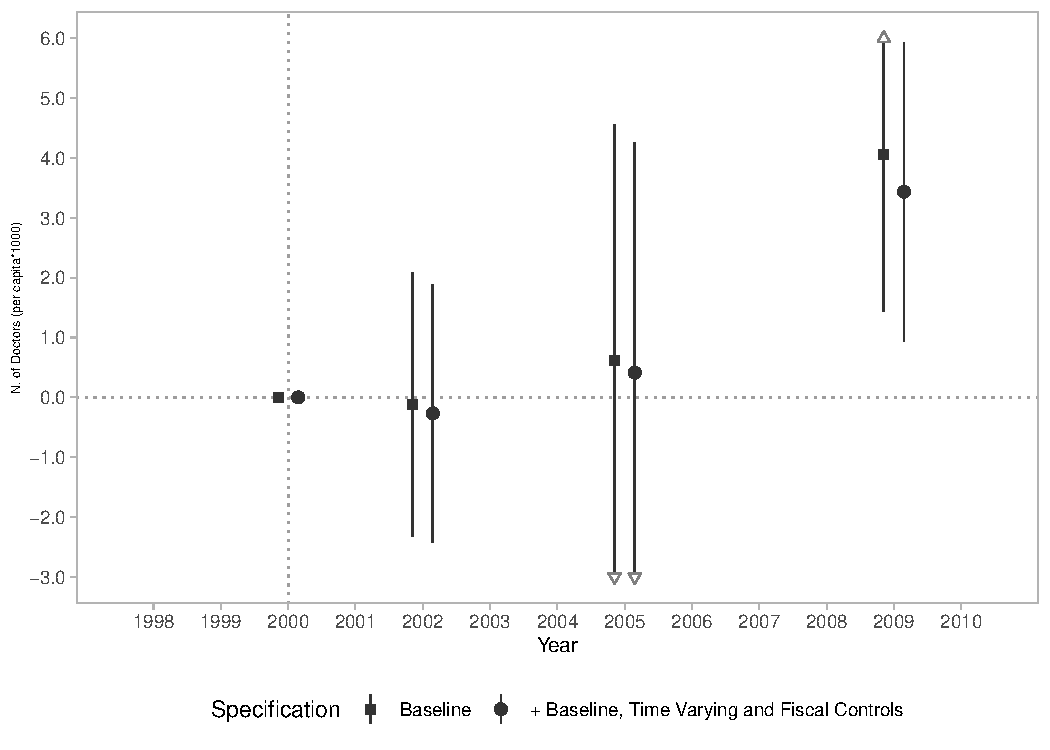
\includegraphics[width=\textwidth]{plots/ams_hr_superior_pcapita_dist_ec29_baseline_dist_ec29_baseline_10.pdf}
    \end{subfigure}
    \begin{subfigure}{0.48\textwidth}
        \centering
        \caption{\scriptsize Number of Nurses (per capita*1000)}\label{fig:10b}
        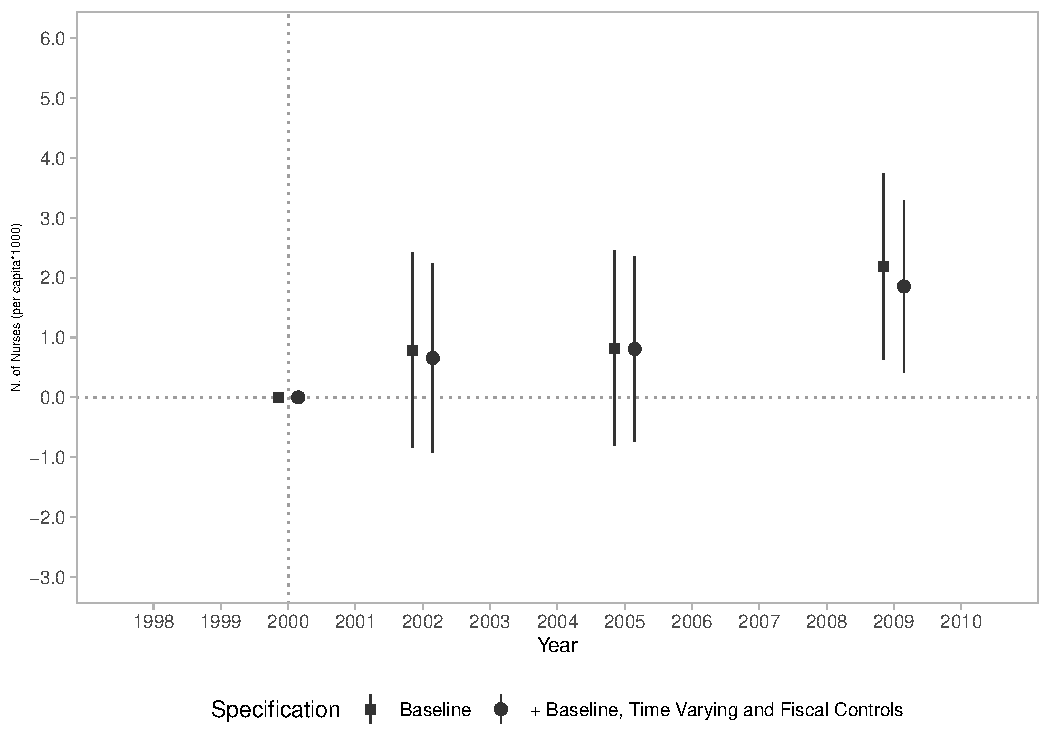
\includegraphics[width=\textwidth]{plots/ams_hr_technician_pcapita_dist_ec29_baseline_dist_ec29_baseline_10.pdf}
    \end{subfigure}
    \begin{subfigure}{0.48\textwidth}
        \centering
        \caption{\scriptsize Number of Nursing Assistants (per capita*1000)}\label{fig:10c}
        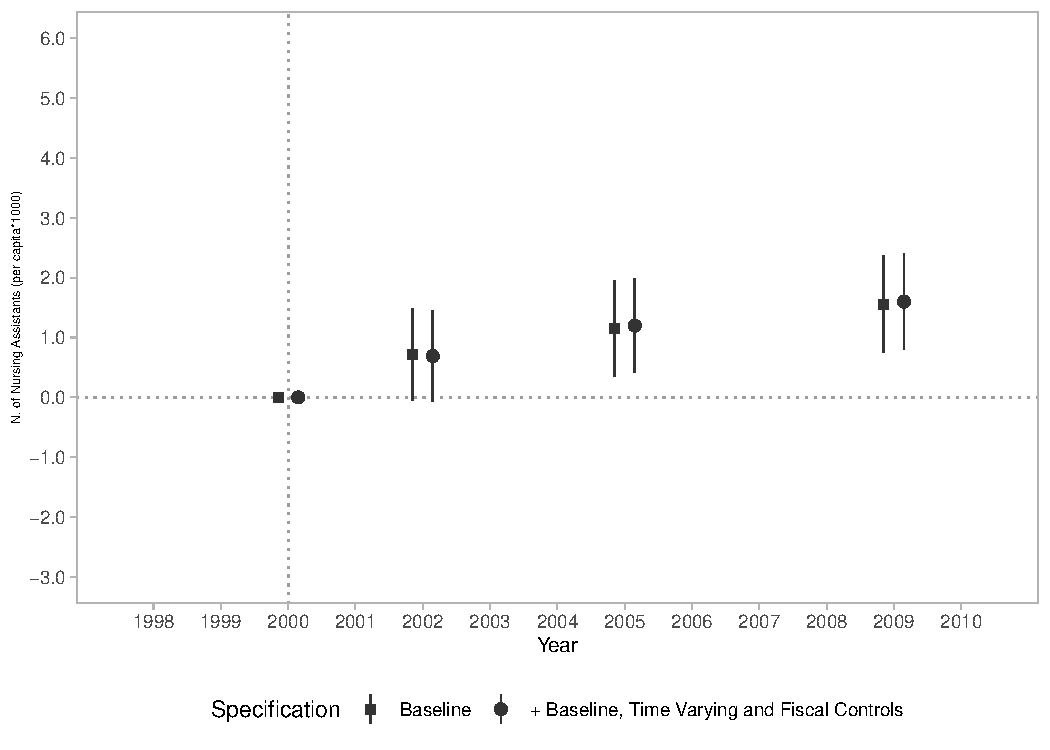
\includegraphics[width=\textwidth]{plots/ams_hr_elementary_pcapita_dist_ec29_baseline_dist_ec29_baseline_10.pdf}
    \end{subfigure}
    \begin{subfigure}{0.48\textwidth}
        \centering
        \caption{\scriptsize Number of Administrative Professionals (per capita*1000)}\label{fig:10d}
        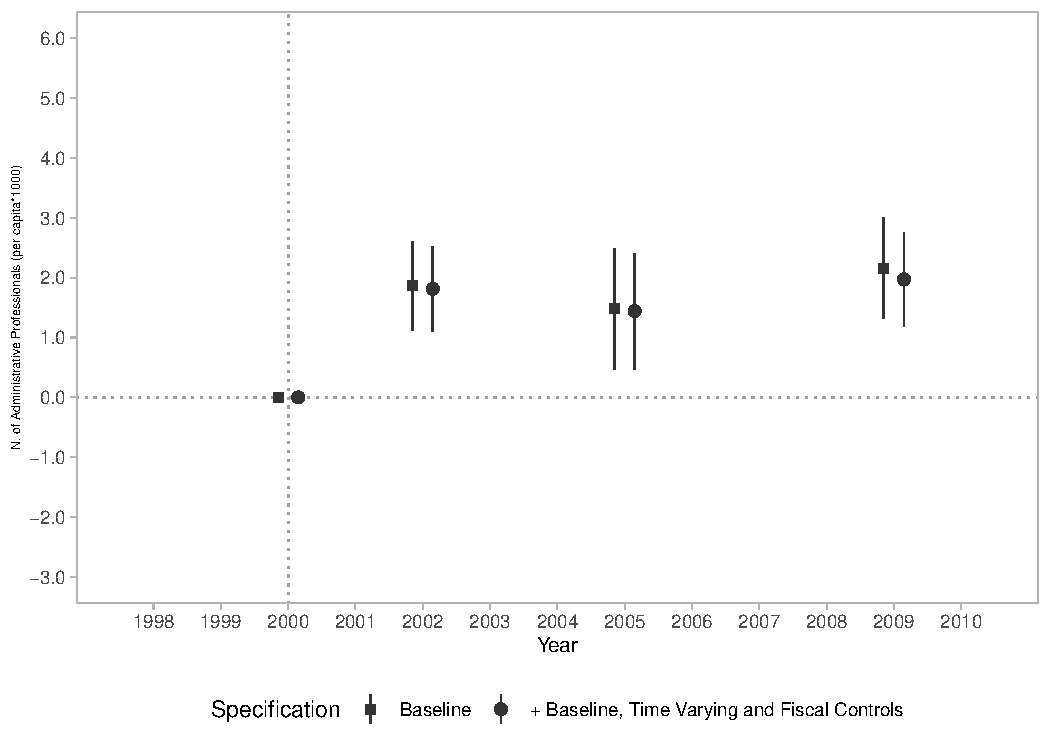
\includegraphics[width=\textwidth]{plots/ams_hr_admin_pcapita_dist_ec29_baseline_dist_ec29_baseline_10.pdf}
    \end{subfigure}
    
    \end{center}
    \scriptsize{Notes: The number of observations is 19364. DiD Estimates from Equation \ref{eq:2}. Independent variable is the distance to the EC/29 target in p.p. Square dots represent the baseline model with municipality and state-year fixed effects. Round dots represent fully saturated specification (Column 4 in regression Tables). Lines represent 95\% confidence intervals. Arrows, when present, indicate confidence intervals out of the plot bounds. Standard errors are clustered in the municipality level.}
    
\end{figure}